\section{Introduction}

Event recognition and detection in videos has hugely benefited from the
introduction of recent large-scale datasets \cite{THUMOS,UCF101,Karpathy_CVPR14,MED11} and models.
However, this is mainly confined to the domain of single-person actions
where the videos contain one actor performing a primary activity.
Another equally important problem is event recognition in
videos with multiple people. In our work, we present a new model
and dataset for this specific setting.

\begin{figure}[ht!]
\begin{center}
  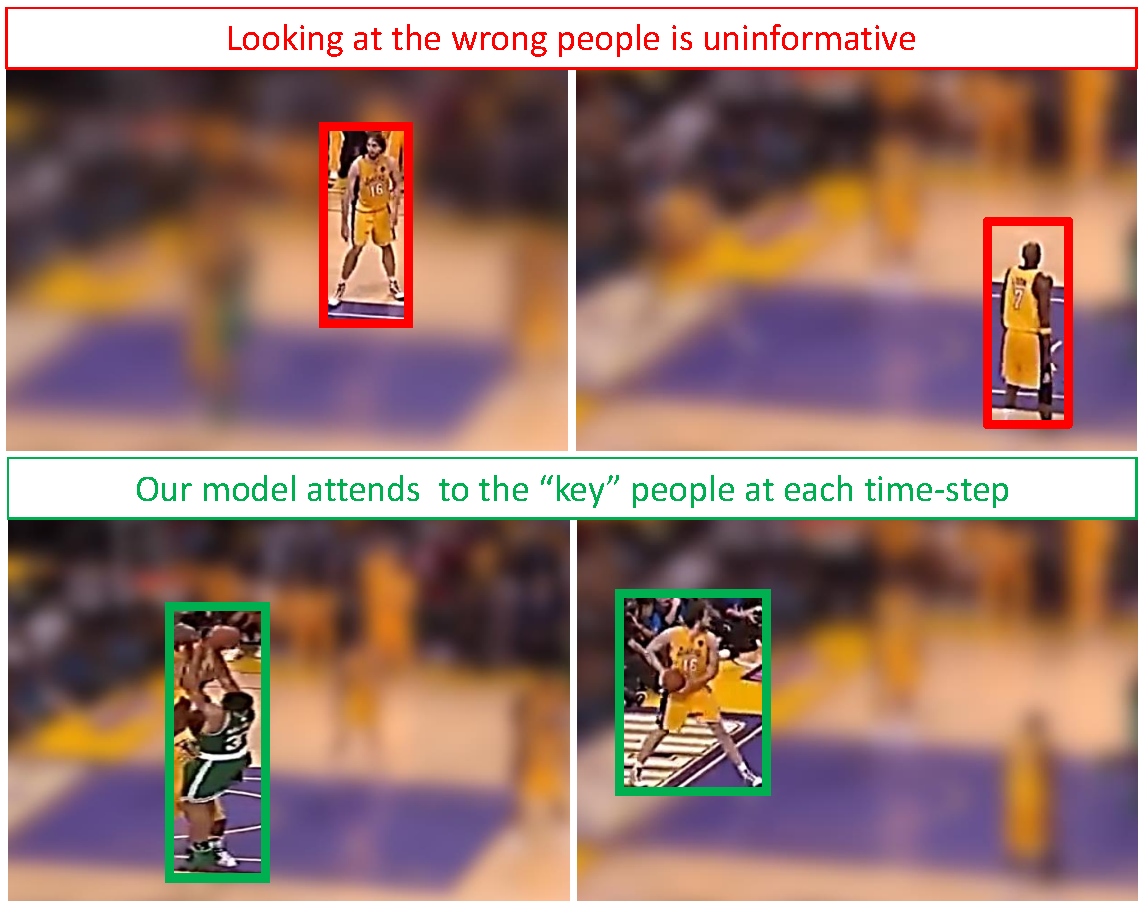
\includegraphics[width=3.2 in]{images/pull_figure_v3_cropped.pdf}
\end{center}
\caption{Looking at the wrong people in a multi-person event can be very uninformative
  as seen in the first row. However, by observing the correct people in the same video
  (second row), we can easily identify the event as a ``2-pointer success" based
  on the shooter and
the player throwing the ball into play. Our model uses this intuition
to recognize the key players for event recognition.}
\label{fig:pull_figure}
\end{figure}

Videos captured in sports arenas, market places or other outdoor areas
typically contain multiple people interacting with each other.
Typically most people are doing ``something'', but not all of them are involved in the main event.
The main events is dominated by a smaller subset. For instance, a ``shot" in a game
or ``shop-lifting" in a market is determined by one or two key people.
Apart from recognizing the event it is also important
to isolate these key actors. This is a significant challenge which
differentiates multi-person videos from single-person videos.

Identifying the people responsible for the event is an interesting task in its
own right.  It is also desirable to learn a model which does not require
annotations for identifying these people during training. \VIGNESH{ This can
also be viewed as a problem of weakly supervised key player identification.} In
this paper, we propose a method  to classify events by using a model that is
able to ``attend'' to a subset of the key people.  We  do this without ever
explicitly telling the model who or where the key people are.

Recently, several papers have proposed to use ``attention" models for aligning
elements from a fixed input to a fixed output.  For example,
\cite{Bahdnau_arxiv14} translate sentences in one language to another language,
attending to different words in the input; \cite{Xu_arxiv15} generate an image-caption,
attending to different regions in the image; and
\cite{Yao_arxiv15} generate a video-caption, attending to different
frames within the video.  In these settings, the input sequence remains fixed
at all times and the model chooses from this fixed input at each instant.
\JONATHAN{Fix discontinuitiy here.}

In our work, we use attention to decide which of several people is most
relevant to the action being performed; this attention mask can change over
time. Thus we are combining spatial and temporal attention.  Note that while
the person detections vary from one frame to another, they can be associated
across frames through tracking. We provide an RNN based representation for the
tracks and the attention model is tasked with selecting from this
representation. We show that this results in improved event recognition
performance.

In order to evaluate our method, we need a large number of videos illustraintg
events involving multiple people. Most prior activity and event
recognition datasets focus on actions involving just one or two people.
Multi-person datasets like \cite{Ryoo_ICCV09,VIRAT,Choi_ICCV09} are usually restricted to fewer videos.
Therefore we decided to collect our own dataset.
In particular we collect a new dataset of basketball events with time-stamp annotations for
all occurrences of $11$ different events across $257$ videos each $1.5$ hours
long in length.  This dataset is comparable to the THUMOS \cite{THUMOS}
detection dataset in terms of number of annotations, but contains longer videos
in a multi-person setting.

In summary, the contributions of our are paper are as follows.  First, we
introduce a new  large-scale basketball event dataset with 14K dense temporal
annotations for long video sequences.  Second, we show that our method
outperforms state-of-the-art methods for the standard tasks of classifying
isolated clips and of temporally localizing events within longer, untrimmed
videos.  Third, we show that our method learns to attend to the relevant
players, despite never being told which players are relevant in the training
set.
